\chapter{Up To Five Sort}
\label{cha:up to five sort}


  \section{Lexicographic Smallest}
  \label{sec:utfs_lexicographic_smallest}
    LexicographicSmallest was not changed for ImprovedNearestNeigbor, for analysis of this function see \ref{sec:nn_lexicographic_smallest}.

  \section{Insert Lost Points}
  \label{sec:utfs_insert_lost_points}

    \subsection{Definitions}
    \label{sub:ilp_definitions}
        \begin{definition} \label{def:ilp}

        \end{definition}

    \subsection{Functional Description}


    \subsubsection{Proof of Correctness}
    \label{ssub:ilp_proof}

    \subsection{Running Time Analysis}
    \label{sub:ilp_running_time_analysis}

  \section{Up To Five Sort}
  \label{sec:up to five sort}

    \subsection{Definitions}
    \label{sub:utfs_definitions}
      \begin{definition} \label{def:inn}

      \end{definition}

    \subsection{Functional Description}
    \label{sub:utfs_functional_description}


    \subsubsection{Proof of Correctness}
    \label{ssub:utfs_proof}

    \subsection{Running Time Analysis}
    \label{sub:utfs_running_time_analysis}


  \section{Test Results}
  \label{sec:utfs_test_results}
    \subsection{Running time}


        \begin{table}[!h!b!p]
        \begin{center}
          \begin{tabular}{|p{2.5cm}|p{2.5cm}|}
              \hline
              Points & Seconds\\
              \hline
              \hline
              500 & 0.015\\
              \hline
              1000 & 0.031\\
              \hline
              1500 & 0.041\\
              \hline
              2000 & 0.078\\
              \hline
              5000 & 0.390\\
              \hline
              10000 & 1.747\\
              \hline
              15000 & 5.008\\
              \hline
              20000 & 8.783\\
              \hline
              30000 & 20.951\\
              \hline
              40000 & 25.053\\
              \hline
              50000 & 53.991\\
              \hline
              60000 & 71.230\\
              \hline
              80000 & 139.543\\
              \hline
          \end{tabular}
          \label{tab:utfs_runningtime}
          \caption{Results of testing ImprovedNearestNeighbor}
        \end{center}
      \end{table}


        \begin{figure}
          \begin{center}
            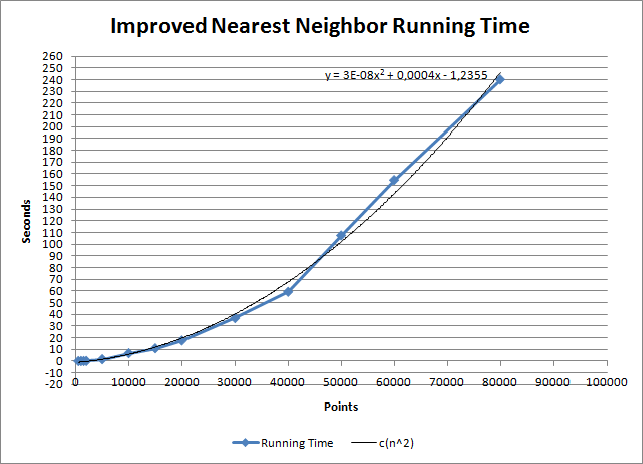
\includegraphics[scale = 0.7]{3ImprovedNearestNeighbor/innRuntimeGraph.png}\\
            \caption{Graph of Improved Nearest Neighbor Running Time}
            \label{fig:inn_runnningtime}
          \end{center}
        \end{figure}

      \noindent The results of the running

    \subsection{Correct output}


   \subsection{Conclusion from tests} 